\documentclass{article}
\author{Austin Hall}
\date{March 2020}
\title{\huge Sun-Data Analysis}
\usepackage{natbib}
\usepackage{graphicx}
\usepackage{amsmath}
\usepackage{epstopdf}
\usepackage{setspace}
\usepackage{indentfirst}

\doublespacing
\begin{document}
\maketitle
\begin{center}
{\LARGE Abstract}\\
\end{center}

\newpage
\section{Introduction}
\par While the relationship between sunspots and cosmicrays is well established,
the exact mechanism of this connection is lightly know compared to their
statistical connection. In this data analysis project the aim was to visualy
and quanitatively represent the cause-affect relationship of sunspots with
cosmic rays.\\
\par To acheive this, data for a specific time interval and region was 
obtained from the NOAA repositories affording a quanitative analysis.\cite{raydata} \cite{spotdata}
Sunspots are tabulated through the use of the Wolf number: $R_z=k(10g+s)$.
Where $k$ is the scaling factoring varying for location and types of intrumentation.
While $g$ representsthe number of sunspot groups and $s$ represents the number
of individual sunspots.\\
\par Using python, each data-set was filtered and
restructed for analysis. The data reflects and indirect correlation between
sunspots and cosmicray. Also, in quanitateing the correlation time between
each corresponding maximum and minimum yielded an average suggesting
a statistical gap between the two occurances.


\newpage
\section{Methods}
\par Using the files from the NOAA repository the data files were read and 
restructured with python to remove extraneous data.
Sunspots are tabulated through the use of the Wolf number: $R_z=k(10g+s)$.
Where $k$ is the scaling factoring varying for location and types of intrumentation.
While $g$ represents the number of sunspot groups and $s$ represents the number
of individual sunspots.\\

\par After proper structuring
the data was then smoothed through the use of a moving average since the 
original files contain high fluctuations within the data set.
The moving average data-set was utilized in two manners. 
Visual use came through the contruction of a subplot representing
cosmic-rays and sunspots over the course of a $50$ year period. Then was used
numerically to determine the relative maximum's and minimum's within a time
period. After determining the relative extrema the time difference between
their occurances was tabulated and averaged. 


\newpage
\section{Results}
\begin{figure}[h!]
\centering
\caption{plot}
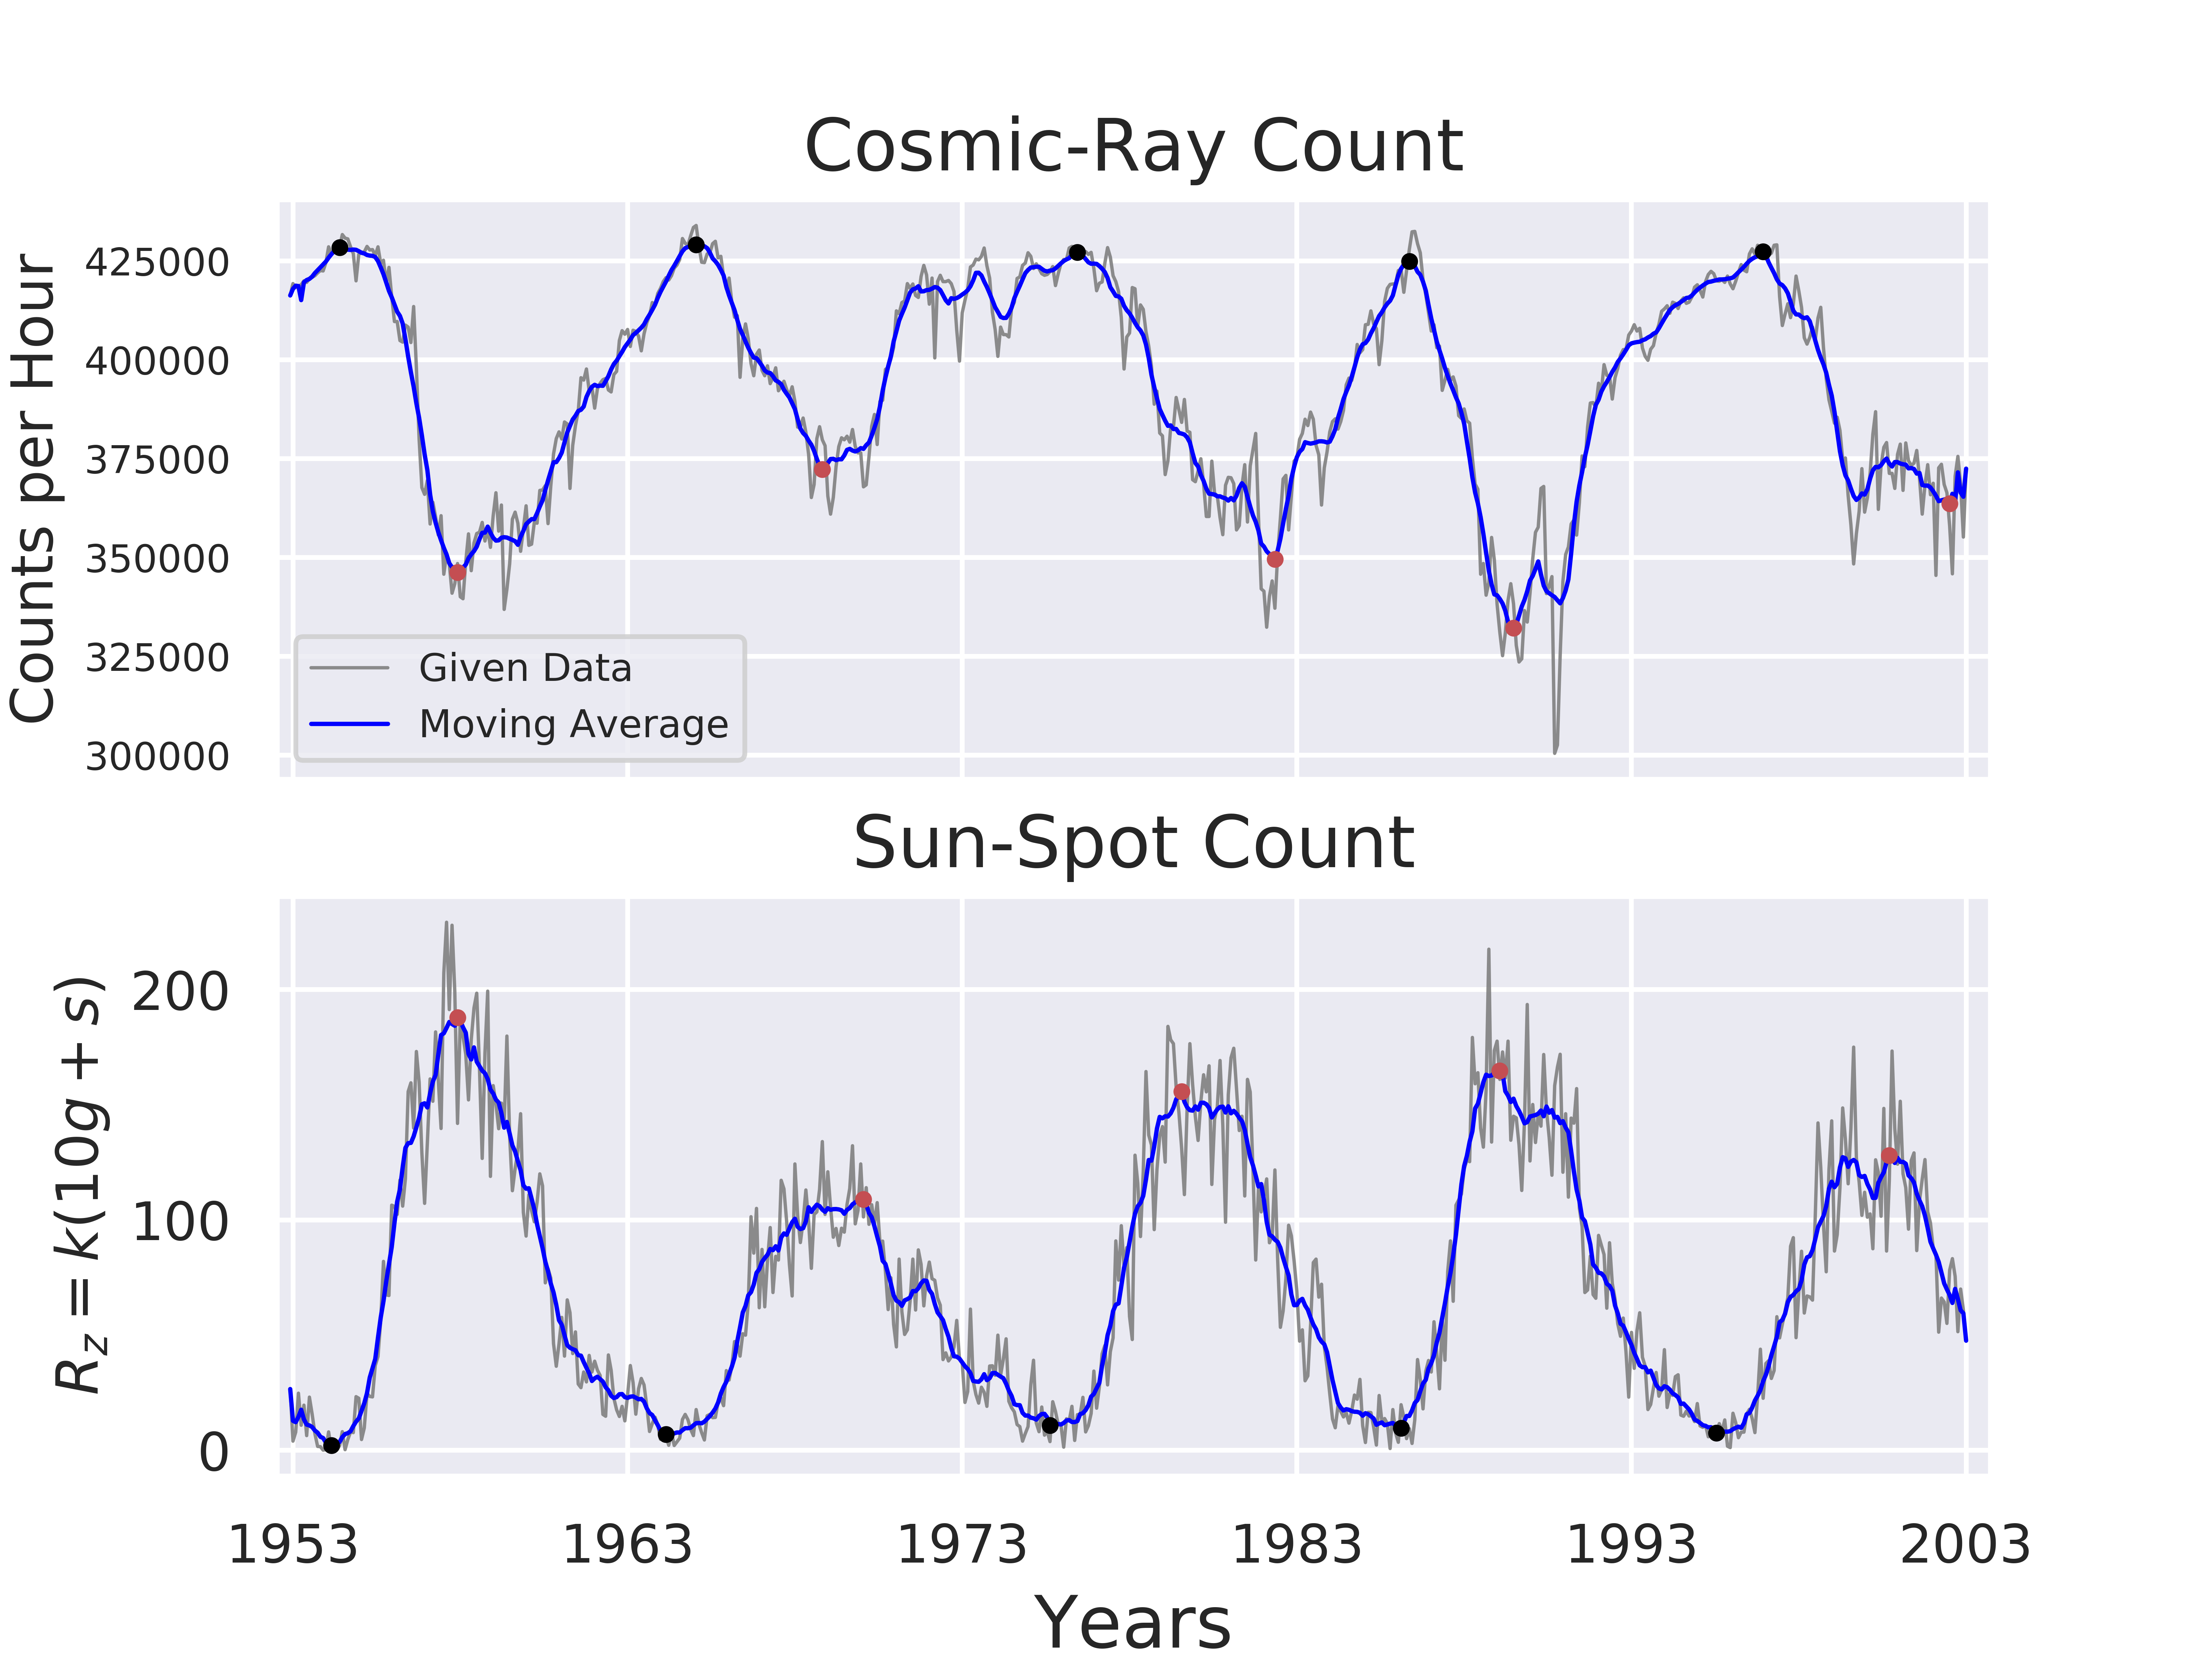
\includegraphics[scale=0.7]{plot.png}
\label{fig:sundata}
\end{figure}
\begin{table}[h!]
 \centering
 \small
 \caption{table}
 \label{tbl:timelag}
 \begin{tabular}{| p{2cm} |p{2cm} |p{1cm}||p{2cm}|p{2cm}|p{1cm}|  }
  \hline
  \multicolumn{6}{|c|}{Time-Gap Data Avg=8.4 Months} \\
  \hline
  Cosmic-Ray Max's&Sun-Spot Min's&Time Gap&Cosmic-Ray Min's&Sun-Spot Max's&Time Gap\\
  \hline
  July,1954&April,1954&-3 Months&February,1958&February,1958&0 Months\\
  May,1965&June,1964&-11 Months&March,1969&June,1970&+10 Months\\
  December,1976&February,1976&-10 Months&December,1982&February,1980&-34 Months\\
  January,1987&October,1986&-3 Months&February,1990&October,1989&-4 Months\\
  October,1997&May,1996&-7 Months&June,2003&August,2001&-22 Months\\
  \hline
 \end{tabular}
\end{table}
\newpage
\section{Analysis}


\newpage
\section{Conclusion}
\newpage
\bibliographystyle{plain}
\bibliography{bib.bib}

\end{document}
